\documentclass[../main]{subfiles}

%TeXromancers title page template
%by derivada.schwarziana

\begin{document}

%please update these for each book release:

\newcommand{\bookauthor}{Daniel Quillen}
\newcommand{\shortbookauthor}{Quillen}
\newcommand{\booktitle}{Homotopical Algebra}
\newcommand{\booksubtitle}{}

\newcommand{\bookcoverTeXromancers}{Revised and modernized edition by}

\newcommand{\bookcoverpicture}{
\scalebox{3}{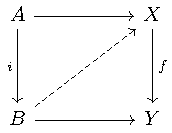
\includegraphics{cover/QHA_cover.pdf}}

}

\newcommand{\bookoriginaledition}{1965}
\newcommand{\bookthisedition}{2022}

%these are meant for the back cover
%both should have ~100 words
\newcommand{\bookreview} 
{
Daniel Quillen, 1940–2011, Fields Medalist, transformed many aspects of algebra, geometry, and
topology. Especially in a succession of remarkable
papers during the ten-year period of 1967–1977,
Quillen created astonishing mathematics which
continues to inspire current research in many
fields. Quillen’s mathematical exposition serves
as the ultimate model of clarity. Despite his
brilliance, those who knew Quillen were regularly impressed by his generosity and modesty
}

\newcommand{\bookauthorbio}
{
}
\newcommand{\authorbiosource}{Memorium article, edited by Eric Friedlander and Daniel Grayson}     %BOOK INFO GOES HERE -- please update _BOOKINFO.tex for new books
%http://paletton.com/#uid=b14333r0kkAw01RZWclMishq8B4eb

\definecolor{tyellow}{HTML}{FFD05B}
\definecolor{tyellowlight}{HTML}{FFE39D}
\definecolor{tyellowlighter}{HTML}{FFFBF0}
\definecolor{tyellowdark}{HTML}{D09B18}
\definecolor{tyellowdarker}{HTML}{715000}

\definecolor{tturq}{HTML}{3EAF7F}
\definecolor{tturqlight}{HTML}{86DAB6}
\definecolor{tturqlighter}{HTML}{EEFCF6}
\definecolor{tturqdark}{HTML}{118F59}
\definecolor{tturqdarker}{HTML}{004D2C}

\definecolor{tblue}{HTML}{3E83A1}
\definecolor{tbluelight}{HTML}{86BCD4}
\definecolor{tbluelighter}{HTML}{EEF8FC}
\definecolor{tbluedark}{HTML}{156283}
\definecolor{tbluedarker}{HTML}{033247} %colors

%title page
\newpage
\thispagestyle{empty}


\begin{tikzpicture}[remember picture,overlay]
%uses the calc library
    \node (title)
        [shape=rectangle, 
         outer sep=2em,
         inner sep=2em,
         minimum height=18em, 
         minimum width=\paperwidth, 
         align=flush right, 
         text=black,
         text width=0.8\paperwidth,
         anchor=north
        ] 
        at ($(current page.center)!0.6!(current page.north)$)
        {
        \fontsize{5em}{4em}
        \fontfamily{lmss}
        \selectfont
        \booktitle\par
        };
        
    \node (author)
        [
         inner sep=0.75em,
         align=flush right,
         text=black,
         anchor=east
        ]
        at ($(title.north east)-(0.125\paperwidth,0)$)
        {
        \fontsize{3em}{2.5em}
        \fontfamily{lmss}
        \selectfont
        \bookauthor\par
        };
    \node (coverinfo)
        [text=black]
        at ($(current page.center)!0.825!(current page.south)$)
        {
        \fontsize{1.5em}{1em}
        \fontfamily{lmss}
        \selectfont
        \bookcoverTeXromancers\par
        };
    \node
        [text=black]
        at ($(current page.center)!0.9!(current page.south)$)
        {
        
\includegraphics[height=3em]{texromancers_gray.pdf}
        \raisebox{1.1em}{
        \fontsize{1.5em}{1em}\selectfont\TeX{}romancers\par
        }
        };
\end{tikzpicture}

\end{document}